\section{商空间回顾}
\sourcepage{129--130}
本节复习商空间的一些基本概念。

若满射 $p:X\to Y$ 满足：$U\subset Y$ 为开集，当且仅当 $p^{-1}(U)$ 在 $X$ 中开，则称为\textbf{商映射}（quotient map）。等价地，也可要求 $E$ 在 $Y$ 中闭，当且仅当 $p^{-1}(E)$ 在 $X$ 中闭。

若 $X$ 的子集 $C$ 等于某个 $A\subset Y$ 的完整原像 $p^{-1}(A)$，则称 $C$ 关于 $p$ \textbf{饱和}（saturated）。$p$ 为商映射，等价于 $p$ 连续，并把饱和开集映为开集；也等价于把饱和闭集映为闭集。

若连续满射 $p$ 为开映射或闭映射，则它为商映射。特别地，若 $X$ 紧致、$Y$ 为 Hausdorff 空间，则 $p$ 为闭映射，因而是商映射。

先列出若干初等事实，证明直接，留给读者。
\begin{itemize}
\item 一一的商映射为同胚。
\item 商映射的复合仍为商映射。
\item 商映射的限制有时仍为商映射：若 $A\subset X$ 饱和，且在 $X$ 中开或闭，则 $p$ 在 $A$ 上的限制为商映射。
\end{itemize}
商映射与连续映射的关系如下：若 $p:X\to Y$ 为商映射，$f:X\to Z$ 连续，且在每个纤维 $p^{-1}(y)$ 上为常值，则存在唯一连续映射 $g:Y\to Z$，使 $gp=f$。称 $g$ 为 $f$ \textbf{诱导的映射}。

如下定义商空间。设 $X^*$ 为将 $X$ 分成两两不交子集的一个划分，令 $\pi:X\to X^*$ 将每点映到包含它的那个子集。规定 $U\subset X^*$ 为开集，当且仅当 $\pi^{-1}(U)$ 在 $X$ 中开，得到 $X^*$ 上的拓扑。此时 $\pi$ 为商映射，称 $X^*$ 为 $X$ 的\textbf{商空间}。常说它由将划分中的每个成员等同为一点而得到。

若 $p:X\to Y$ 为商映射，可按如下方式把 $Y$ 视为 $X$ 的商空间：用各纤维 $p^{-1}(y)$ 划分 $X$，所得 $X^*$ 与 $Y$ 同胚。事实上，利用前面的诱导映射性质，分别得到 $g:X^*\to Y$、$h:Y\to X^*$，满足 $g\pi=p$、$hp=\pi$；容易看出它们互逆。

\entry{例}{2.8.1}将 $x$-$z$ 平面内以 $(2,0,0)$ 为中心的单位圆绕 $z$ 轴旋转，得到 $\R^3$ 的子空间 $X$。用柱坐标 $(r,\theta,z)$，它由方程 $(r-2)^2+z^2=1$ 表示。令 $I^2=I\times I$，对 $(s,t)\in I^2$，按
\[
r-2=\cos2\pi t,\qquad z=\sin2\pi t,\qquad\theta=2\pi s
\]
定义 $p:I^2\to X$。可验证它为满的闭商映射。因此 $X$ 可视为将 $(s,0)$ 与 $(s,1)$、$(0,t)$ 与 $(1,t)$ 分别等同而得的商空间，见图 2.8.1。这是第 1.4 节粘合矩形各边构造环面的拓扑表述。
\begin{center}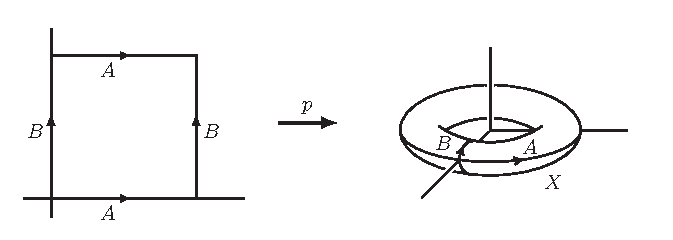
\includegraphics[width=117mm]{figures/2-8-1.pdf}\\图 2.8.1\end{center}

\sourcepage{131--132}
分离公理在商空间中不一定保持，例如 Hausdorff 空间的商空间未必 Hausdorff。一般只能说：若每个纤维 $p^{-1}(y)$ 都在 $X$ 中闭，则 $Y$ 为 $T_1$ 空间，即单点集闭。因此，若 $X^*$ 是将 $X$ 划分为闭集的划分，所得商空间为 $T_1$ 空间。\translatornote{原文还插入一句“若 $X$ 为 Hausdorff，则 $Y$ 的单点集闭”；单有该假设不足，仍须保留纤维闭的条件。}

后面会更详细地讨论商空间的分离公理。这里最后讨论：两个商映射的笛卡尔积何时仍为商映射？有两个相关结果。

\entry{定理}{2.8.2}若 $p:X\to Y$ 为商映射，$C$ 为局部紧致 Hausdorff 空间，则 $p\times i_C:X\times C\to Y\times C$ 为商映射。

\noindent\textbf{证明：}令 $\pi=p\times i_C$。设 $A\subset Y\times C$ 且 $\pi^{-1}(A)$ 开，证明 $A$ 开。给定 $(y_0,c_0)\in A$，选 $x_0$ 使 $p(x_0)=y_0$。可选择 $x_0,c_0$ 的开邻域 $U_1,W$，使 $U_1\times W\subset\pi^{-1}(A)$。由局部紧致 Hausdorff 性，选 $c_0$ 的开邻域 $V$，使 $\overline V$ 紧致且 $\overline V\subset W$。于是
\[
U_1\times\overline V\subset\pi^{-1}(A).
\]
一般地，若已构造开邻域 $U_i$，使 $U_i\times\overline V\subset\pi^{-1}(A)$，则 $p^{-1}p(U_i)$ 虽未必开，却包含 $U_i$。构造开集 $U_{i+1}$，使
\[
p^{-1}p(U_i)\times\overline V\subset U_{i+1}\times\overline V\subset\pi^{-1}(A).
\]
对每个 $x\in p^{-1}p(U_i)$，有 $\{x\}\times\overline V\subset\pi^{-1}(A)$。由紧致性，可取开邻域 $W_x$，使 $W_x\times\overline V\subset\pi^{-1}(A)$。令 $U_{i+1}=\bigcup_xW_x$ 即可，见图 2.8.2。
\begin{center}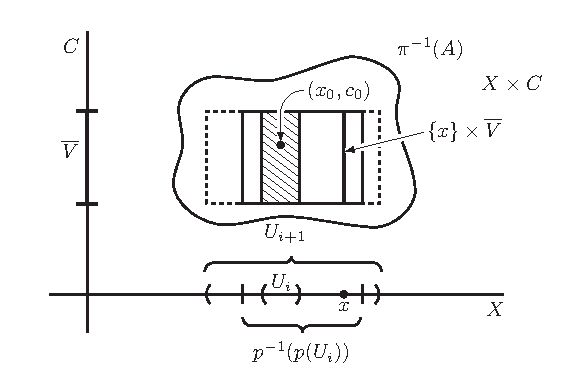
\includegraphics[width=103mm]{figures/2-8-2.pdf}\\图 2.8.2\end{center}
最后令 $U=\bigcup_iU_i$。它开，$U\times V$ 是 $(x_0,c_0)$ 的邻域，并包含于 $\pi^{-1}(A)$。此外，
\[
U\subset p^{-1}p(U)=\bigcup_i p^{-1}p(U_i)=\bigcup_iU_{i+1}=U,
\]
故 $U$ 饱和，$p(U)$ 在 $Y$ 中开。于是 $p(U)\times V=\pi(U\times V)\subset A$ 是 $(y_0,c_0)$ 的开邻域，证毕。\hfill$\square$

\entry{推论}{2.8.3}若 $p:A\to B$、$q:C\to D$ 为商映射，且 $p$ 的定义域 $A$ 与 $q$ 的值域 $D$ 均为局部紧致 Hausdorff 空间，则 $p\times q:A\times C\to B\times D$ 为商映射。

\noindent\textbf{证明：}写成复合 $A\times C\xrightarrow{i_A\times q}A\times D\xrightarrow{p\times i_D}B\times D$，两映射均为商映射，复合亦然。\hfill$\square$

相干拓扑与商映射有密切关系，描述如下。

\sourcepage{133}
\entry{定义}{2.8.4}设空间 $E$ 是两两不交子空间 $E_\alpha$ 的并，且每个 $E_\alpha$ 在 $E$ 中开且闭，则称 $E$ 为它们的\textbf{拓扑和}（topological sum），记为 $E=\coprod E_\alpha$。集合 $U$ 在 $E$ 中开，当且仅当每个 $U\cap E_\alpha$ 在 $E_\alpha$ 中开。

更一般地，对未必互不相交的空间族 $\{X_\alpha\}_{\alpha\in J}$，令 $E_\alpha=X_\alpha\times\{\alpha\}$，以这些不交空间的并为底集，赋予上述拓扑。存在自然投影 $p:E\to\bigcup X_\alpha$，把每个 $X_\alpha\times\{\alpha\}$ 投影到 $X_\alpha$。有时也称 $E$ 为各 $X_\alpha$ 的拓扑和。

\entry{引理}{2.8.5}设 $X$ 为若干子空间 $X_\alpha$ 的并，$E$ 为其拓扑和，$p:E\to X$ 为自然投影。则 $X$ 的拓扑与各 $X_\alpha$ 相干，当且仅当 $p$ 为商映射。

证明立即得到。在此情形，常称 $X$ 为各 $X_\alpha$ 的\textbf{相干并}。

\entry{定理}{2.8.6}若 $X$ 的拓扑与子空间族 $X_\alpha$ 相干，$Y$ 为局部紧致 Hausdorff 空间，则 $X\times Y$ 的拓扑与各 $X_\alpha\times Y$ 相干。

\noindent\textbf{证明：}令 $E=\coprod(X_\alpha\times\{\alpha\})$，$p:E\to X$ 为投影。由前一定理，$p\times i_Y:E\times Y\to X\times Y$ 为商映射。由于 $E$ 为各 $E_\alpha$ 的拓扑和，$E\times Y$ 是各开子空间 $E_\alpha\times Y$ 的不交并，因此为它们的拓扑和。应用引理即得结论。\hfill$\square$

\entry{推论}{2.8.7}$|K|\times I$ 的拓扑与各 $\sigma\times I$（$\sigma\in K$）相干。

\noindent\textbf{证明：}$|K|$ 按定义与其单形相干，而 $I$ 是局部紧致 Hausdorff 空间，事实上紧致，故可用定理。\hfill$\square$

\sourcepage{134--135}
\entry{推论}{2.8.8}若 $w*K$ 为锥，则映射 $\pi:|K|\times I\to|w*K|$，$\pi(x,t)=(1-t)x+tw$，为商映射。它将 $|K|\times\{1\}$ 压缩为点 $w$，其他地方为一一映射。\translatornote{原文此处把被压缩的子集误印为整个 $|K|\times I$。}

\noindent\textbf{证明：}若 $\sigma=v_0\cdots v_n$，以 $w*\sigma$ 表示单形 $wv_0\cdots v_n$。集合在锥中闭，当且仅当与每个 $w*\sigma$ 的交闭；集合在乘积中闭，当且仅当与每个 $\sigma\times I$ 的交闭。因此只需证明限制 $\pi':\sigma\times I\to w*\sigma$ 为商映射。它连续满射，涉及的空间均紧致 Hausdorff，所以成立。\hfill$\square$

此推论启发我们定义任意拓扑空间上的锥。

\entry{定义}{2.8.9}空间 $X$ 上的\textbf{锥} $C(X)$，定义为将 $X\times I$ 的子集 $X\times\{1\}$ 等同为一点所得商空间，此点称为\textbf{锥顶}。形式上，将 $X\times I$ 划分为 $t<1$ 时的各单点集 $\{(x,t)\}$ 与集合 $X\times\{1\}$，取所得商空间。

以下定义用于习题 2。

\entry{定义}{2.8.10}取 $\R^2$ 的两个副本 $\R^2\times\{a\}$、$\R^2\times\{b\}$，当 $x\ne0$ 时等同 $(x,a)$ 与 $(x,b)$，得到的空间称为\textbf{双原点平面}（plane with two origins）。

\subsection*{习题}
\begin{enumerate}
\item 验证本节未证明的商空间结果。
\item \begin{enumerate}[label=(\alph*)]
\item 证明双原点平面的每点都有与 $\R^2$ 某开子集同胚的邻域。
\item 证明双原点平面不是 Hausdorff 空间。
\end{enumerate}
\item \begin{enumerate}[label=(\alph*)]
\item 若 $p:X\to Y$ 为开商映射，$A$ 在 $X$ 中开，证明 $p|_A:A\to p(A)$ 为开商映射。
\item 将“开”换为“闭”，重复 (a)。
\end{enumerate}
\item 若 $p:A\to B$、$q:C\to D$ 为开商映射，证明 $p\times q$ 也是。
\item 若 $X$ 为各 $X_\alpha$ 的相干并，$Y$ 为 $X$ 的开或闭子空间，证明 $Y$ 为各 $X_\alpha\cap Y$ 的相干并。
\item 设 $K,L$ 为复形，$K$ 局部有限，证明 $|K|\times|L|$ 的拓扑与各 $\sigma\times\tau$（$\sigma\in K,\tau\in L$）相干。
\item 证明商映射的拓扑和仍为商映射。
\end{enumerate}
